% 2010 年天津卷文科第 9 题：三角形 ABC 中 AD⊥AB，D 在 BC 上。
% 来源 PDF：普通高考/2010/2010天津文.pdf（上游勘误版），SHA-256 e6b06813e17b7c332b651b8784c8fab0fcad0c8666ea6032a2958917c55307c9。
% 原页：第 1 页（A3 四栏）第 2 栏中部，书页码 637。
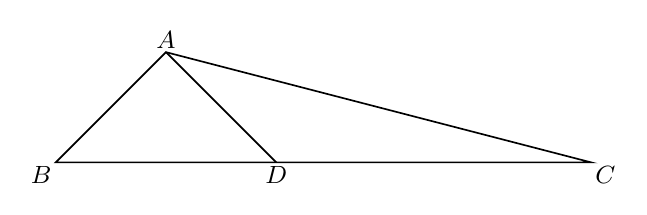
\begin{tikzpicture}[semithick, every node/.style={inner sep=1.2pt, font=\small}]
  \coordinate (A) at (-1.2,1.4);
  \coordinate (B) at (-2.6,0);
  \coordinate (D) at (0.2,0);
  \coordinate (C) at (4.2,0);
  \draw (A) -- (B) -- (C) -- cycle;
  \draw (A) -- (D);
  \node[above] at (A) {$A$};
  \node[below left] at (B) {$B$};
  \node[below] at (D) {$D$};
  \node[below right] at (C) {$C$};
\end{tikzpicture}
